\documentclass{gd-llncs}
%\documentclass[preprint,3p,12pt]{elsarticle}

\usepackage{graphicx}
\usepackage[]{subfig}
\usepackage{svg}
\usepackage[]{pdfpages}
\usepackage[]{svg}
\usepackage{algorithm}
\usepackage{algpseudocode}

\graphicspath{{./images/}}
% \journal{Computational Geometry: Theory and Applications}

%\newtheorem{theorem}{Theorem}
%\newtheorem{problem}{Problem}
%\newtheorem{lemma}{Lemma}
%\newtheorem{proposition}{Proposition}
%\newenvironment{proof}{\noindent \emph{Proof}: }{\qed}

\newcommand{\comm}[1]{}
\newcommand{\TODO}[1]{{\color{magenta}{#1}}}
\newcommand{\new}[1]{\textcolor{green}{#1}}
%\newcommand{\note}[1]{\textcolor{blue}{[#1]}}

\newcommand{\df}[1]{\mbox{\textbf{#1}}}
\def\Cost{\text{\emph{routing cost}}}
\def\aCost{\text{\emph{additional cost}}}
\newcommand{\gv}{\widetilde{G}}
\newcommand{\ink}{I}
\newcommand{\cc}{C}
\newcommand{\inkcoeff}{k_{\textit{ink}}}
\newcommand{\lencoeff}{k_{\textit{len}}}
\newcommand{\capcoeff}{k_{\textit{cap}}}
\DeclareMathOperator{\nul}{\textit{null}}
\newcommand{\cdt}{$\mathcal{T}$}
\newcommand{\unpath}{$\mathcal{L}$}
\newcommand{\triset}{$\mathcal{U}$}
\newcommand{\plg}{$\mathcal{P}$}
\newcommand{\obst}{$\mathcal{O}$}
\newcommand{\capac}{$\mathcal{C}$}
\newcommand{\mw}{$\mathcal{W}$}
\newcommand{\mh}{$\mathcal{H}$}
\begin{document}


\title{Browsing large graphs with XJS, a graph drawing tool in JavaScript }
\author{%
  auth0  \and
  auth1
}%
\institute{
  Institute, US,\\
  \email{auth0@hotmail.com, auth1@gmail.com},\\
  X github home page:
  \texttt{https://github.com/X}
}
\maketitle

\begin{abstract}
  There has been progress in visualization of large graphs recently. Tools appeared that can render a huge graph in seconds. However, if we request that the node labels are visible, and the edges are routed around the nodes, then the problem remains difficult. Interacting with a large graph in an Internet browser with the same ease as browsing an online map is still a challenging task.
In this paper we describe a few novel approaches to large graph visualization that we developed in an open-source JavaScript software.

We give a new efficient edge routing algorithm, where the edges are routed around the nodes. The algorithm produces edge paths which are visually appealing and shortest in their homotopy class.

To facilitate graph visualization with WebGL, or any other platform supporting tiles, we propose a new simple and efficient tiling method. The method guarantees that in every view, except of the highest level, the number of visible entities per tile is not larger than a predefined bound.

We make the node labels of the most important nodes of the current view visible.

The edge routing algorithm mentioned above is reused at the tiling stage to simplify the paths on the lower levels. 
\end{abstract}


\section*{Introduction}

\label{sec:intro}

We target large but not huge graphs. The maximum number of vertices of the graphs we applied our tool at was 28k, 
and the maximum number of the edges was 237k. There are quite a few algorithms that calculate node positions for such graphs, and work very fast~\cite{hu2015visualizing,brandes2007eigensolver}. We look at the node layout, that is an algorithm that only positions the nodes of a graph and does not calculate the edge routes, as a solved problem.

In the first part of the paper we address edge routing where an edge does not intersects the nodes it is not adjacent to. Our approach works for any node layout, as long id does note produce node overlaps.
We build on the edge routing from~\cite{dwyer2010fast} and improve it.
There has been progress in visualization of large graphs recently. Tools appeared that can render a huge graph in seconds. However, the situatiton changes if we request that the node labels are rendered, and the edges overlap only the nodes they are adjacent to. Interacting with a large graph in an Internet browser with the same ease as browsing an online map, inspecting the high level structure and zooming in to the high level detail, is still an unsolved problem. In this paper we describe novel approaches to several aspects of this problem.

We propose a novel and efficient algorithm for edge routing, where each edge can only intersect its source or target. The algorithm produces edge paths which are visually appealing and even optimal in their homotopy class.

To facilitate graph visualization with WebGL, we propose a new simple and fast tiling method. The method guarantees that in every view,
except of the views of the Shighest layer, the number of visible entities is not larger than a
predefined bound. The method can be used in other viewers that support tiling.

Our method provides a high level overview of the graph.

The edge routing algorithm mentioned above is reused at the tiling stage 
to simplify the paths on the lower levels. In addition, we bundle edges per-tile as an optimization heuristic.
Our software runs calculations on the client desktop or a phone, and renders the graph in the browser.
\section*{Related work}
A popular graph drawing tool Graphviz~\cite{graphviz} applies
Scalable Force-Directed Placement~\cite{sfdp} for large graphs, with no
support for tiling. Its edge routing for this case builds the whole
visibility graph. This can be very slow because the visibility graph can have $O(n^2)$ edges,
where $n$ is the number of the nodes in the graph.
Interestingly, the funnel algorithm~\cite{chazelle1982theorem,hershberger1994computing},
the last step of our approach, is used in Graphviz for the edge routing in the
Sugiyama layout. We are not aware of any tool that integrates Graphviz
and uses tiling as well.

yWorks~\cite{yworks} has method "Organic edge routing" that produces edge
routes around the nodes. We could find only
a very general description of the method: "The algorithm is based on a force
directed layout paradigm. Nodes act as repulsive forces on edges in order to
guarantee a certain minimal distance between nodes and edges. Edges tend to contract
themselves. Using simulated annealing, this finally leads to edge layouts that
are calculated for each edge separately". It seems the algorithm runs in $O(n+m)log(n+m)$
time, where $n$ is the number of the nodes and $m$ is the number of the edges.

ReGraph~\cite{regraph} uses WebGL as the viewing platform. It can render a large
graph using straight lines for the edges. The tool does not support tiling, but instead
the user interactively opens the node that is a cluster of nodes.

"graph-tool.skewed"~\cite{skewed} does not implement its own layout algorithms or
edge routing algorithms, but instead provides a nice wrapper around the algorithms from
other layout tools.

Circos~\cite{circos} visualizes large graphs in a circular layout. It does not support tiles.


Cosmograph~\cite{cosmograph} uses a GPU to calculate the layout of a graph and can
handle a graph with a million nodes. It renders edges as straight lines.
It does not support tiling.

The authors of~\cite{nachmanson2015graphmaps} implemented GraphMaps, a tool for large graph visualization. 
The tool only ran in Windows. The edge were routed as polylines on a triangulation. 
The tool supported tiling, but the problem of the limiting number of visible entities was not solved.

In~\cite{perrot2018cornac} an approach to visualize a huge graph is described. The method uses tiles and
edge bundling following~\cite{hurter2012graph}, which is applied at the last moment during the the graph browsing.
The latter calculation is done on the client side, the rest and the majority of the calculations runs on several servers.




\section*{Edge routing in XJS}
The edge routing starts, as in~\cite{dwyer2010fast}, by building a spanner graph, an approximation of the full visibility graph, and then finding shortest paths on the spanner. The spanner, see Fig~\ref{fig:spanner}, is built on a variation of a Yao graph, which was introduced independently by Flinchbaugh and Jones~\cite{flinchbaugh1981strong}  and Yao~\cite{yao1982constructing}. This kind of graph is defined by the set of cones with the apices at the vertices. The cones have the same angle,
usually in the form of $\frac{2\pi} {n}$, where $n$ is a natural number.  The family of cones with the apex at a specific vertex partition the plane as illistrated in Fig.~\ref{fig:yao}. For each cone at most one edge is created connecting the cone apex with a vertex inside of the cone, so the graph has $O(n)$ edges where $n$ is the number of vertices. \\
\begin{figure}[]
  \centering
  \begin{minipage}[b]{0.5\textwidth}
    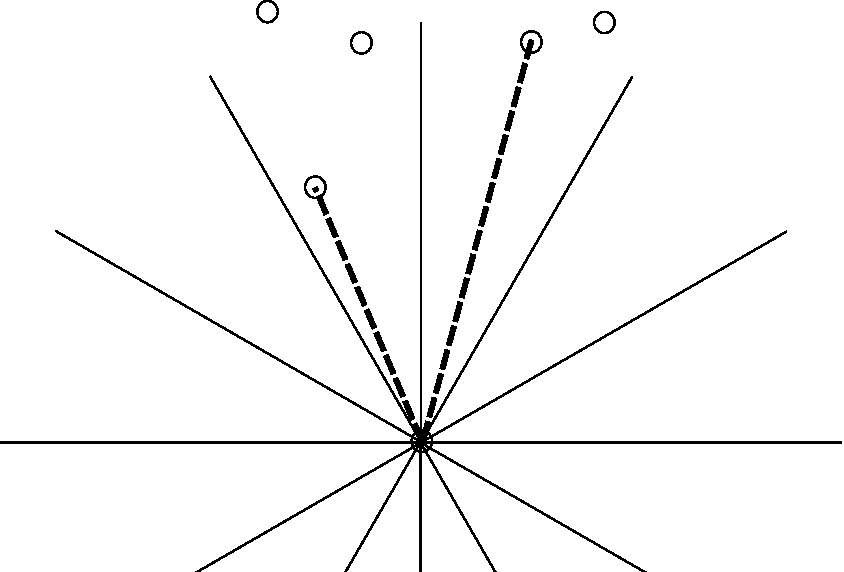
\includegraphics[width=\textwidth]{yao.pdf} 
    \caption{\small{Yao graph}}
    \label{fig:yao}
  \end{minipage}
  \vfill
  \begin{minipage}[b]{\textwidth}
    \includesvg[width=\textwidth]{visibility_graph.svg}
    \caption{\small{Spanner graph is built using the idea of Yao graphs. The dashed curves are the original node boundaries. Each original curve is surrounded by a polygon with some offset to allow the polyline paths smoothing without intersecting the former. \\
        The edge marked by the circles is created because the top vertex is inside of the cone and it is the closest among such vertices to the cone apex. The apex of the cone is the lower vertex of the edge. \\XJS uses cone angle $\frac{\pi}{6}$, so the edges of the spanner can deviate from the optimal direction by this angle. Therefore, the shortest paths on the spanner have length that is at most the optimal shortest length multiplied by $\frac{1}{\cos(\frac{\pi}{6})} \simeq 1.155$.}
    }
    \label{fig:spanner}
  \end{minipage}
\end{figure}

The approach of~\cite{dwyer2010fast} applies local optimizations to shorten an edge path.
Namely, it tries to shortcut one vertex at a time from the path, as illustrated in Fig~\ref{fig:shortcut}.
To smoothen a path, it fits Bezier segments into the polyline corners by
using a binary search to find a larger fitting segment, see Fig~\ref{fig:cornerfit}.
While anylyzing performance of the edge routing in XJS,
we noticed, that for a graph with more than 1k nodes these heuristics
sometime create a performance bottleneck, in spite of using R-Trees\cite{guttman1984r}.
\begin{figure}[!tbp]
  \centering
  \begin{minipage}[b]{0.4\textwidth}
    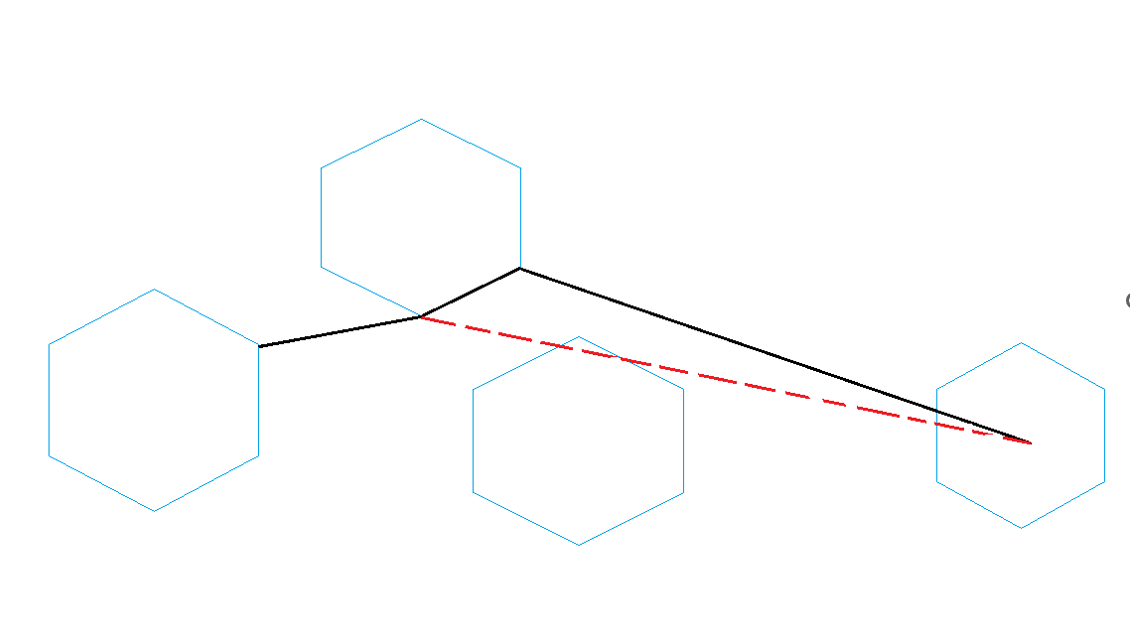
\includegraphics[width=\textwidth]{./naive_shorcut_now_working.png}
    \caption{Unsuccessful shortcut}
    \label{fig:shortcut}
  \end{minipage}
  \hfill
  \begin{minipage}[b]{0.4\textwidth}
    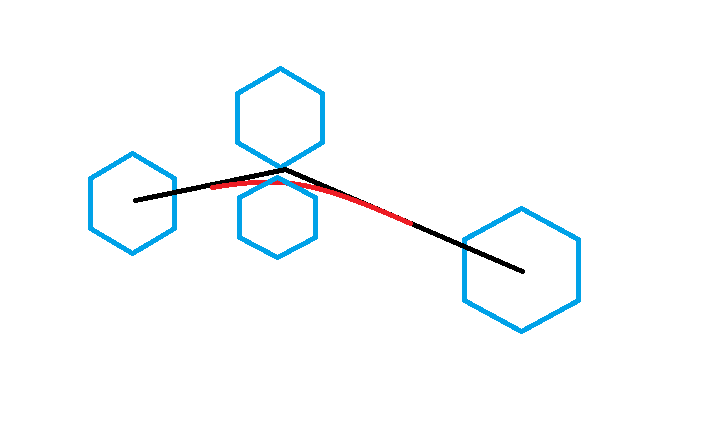
\includegraphics[width=\textwidth]{fillet_corner.png}
    \caption{Fitting a Bezier segment into a polyline corner}
    \label{fig:cornerfit}
  \end{minipage}
\end{figure}
\\
In addition, when the naive shortcutting of polyline corners fails,  the resulting path might remain not visually appealing, as shown in Fig.~\ref{fig:shortcut}.

We replace these heuristics with a more precize and efficient optimization described below.
\subsection*{Path optimization} {
We finalize edge routes by the “funnel” algorithm~\cite{chazelle1982theorem,hershberger1994computing}, routing a path inside a simple polygon, that is a polygon without holes.

An application of the 'path in a simple polygon' optimization to edge routing is not a new idea: the novelty of our work is in how we find the polygon and how we use it.
The authors of Graphvis used the 'funnel' algorithm~\cite{dobkin1997implementing}, but only for hierarchical layouts, where a simple polygon, \plg, containing the path is available. They write: "If \plg~does not contain holes ... we can apply a
standard “funnel” algorithm ... for finding Euclidean shortest paths in a simple polygon". In general case,
for a non-layered layout, they build the visibility graph which is very expensive for a large graph.

Here we find the polygon \plg~for any layout. We drop the requirement that \plg~is simple. Indeed, to run the “funnel” algorithm one only needs a “sleeve”: a sequence of triangles leading from the start to the end of the path, where each triangle shares a side with its successor. Let us show how to build polygon \plg, create a sleeve, and produce an optimized path.

We call obstacles, $\mathcal{O}$, ~the set of polygons covering the original nodes, see Fig.~\ref{fig:spanner}. Before routing edges, we calculate a Constrained Delaunay Triangulation~\cite{delaunay1934sphere} on $\mathcal{O}$. Let us call this triangulation $\mathcal{T}$.

For each edge of the graph we proceed with the following steps.

We route a path, called \unpath, on the spanner, as illistrated by Fig.~\ref{fig:non_opt_path_L}.
\begin{figure}[!tbp]
  \centering
  \begin{minipage}[b]{0.45\textwidth}
    \includesvg[width=\textwidth]{non_optimized_path_on_global_cdt.svg}
    \caption{Path \unpath~with \cdt, a fragment.}
    \label{fig:non_opt_path_L}
  \end{minipage}
  \hfill
  \begin{minipage}[b]{0.45\textwidth}
    \includesvg[width=\textwidth]{poly2.svg}
    \caption{Polygon \plg~containing \unpath.}
    \label{fig:polygon_with_path}
  \end{minipage}
  \vfill
  \begin{minipage}[b]{0.45\textwidth}
    \includesvg[width=\textwidth]{poly3.svg}
    \caption{New triangulation of \plg.}
    \label{fig:new_triangulation}
  \end{minipage}
  \hfill
  \begin{minipage}[b]{0.45\textwidth}
    \includesvg[width=\textwidth]{poly4.svg}
    \caption{The optimized path together with the sleeve diagonals.}
    \label{fig:optimized_path}
  \end{minipage}
\end{figure}
Let $\mathcal{S}$ and $\mathcal{E}$ be the obstacles containing correspondengly \unpath's start and end point.
To obtain \plg, let us consider \triset, the set of all triangles ${t} \in \mathcal{T}$ such that
either ${t} \subset \mathcal{S} \cup \mathcal{E}$, or $t$ intersects \unpath~and is not inside of any obstacle in $\mathcal{O} \setminus \{S,E\}$  .
The union of \triset~gives us \plg. The boundary of \plg~comprizes all sides $e$ of the triangles from \triset~ such that $e$ belongs to exactly one triangle from \triset, see Fig.~\ref{fig:polygon_with_path}. \\
To create the sleeve~\cite{chazelle1982theorem,hershberger1994computing}, we need to have a triangulation of \plg~such that every edge of the triangulation is either a boundary edge of \plg, or a diagonal of \plg. Because \triset~might not have this property, as in Fig.~\ref{fig:polygon_with_path}, we create a new Constrained Delaunay Triangulation of \plg, where the set of constrained edges is the boundary of \plg, see Fig.~\ref{fig:new_triangulation}.\\
We trace path \unpath~through the new triangulation and obtain the sleeve. Finally, we apply the funnel algorithm on the sleeve and obtain the path which is the shortest in the homotopy class of \unpath, as illustrated in Fig.~\ref{fig:optimized_path}.\\
The discussion~\cite{pathOpt} of the algorithm helped us in the implementation.\\
\begin{figure}[]
  \centering
  \includegraphics*[width=0.6\textwidth]{sleeve_diagonals_not_optimal.pdf}
  \caption{\plg~is not simple. The dotted path is shorter than the dashed one that was found by the routing.}
  \label{fig:non_optimal_path}
\end{figure}
Polygon \plg~is not necessarily simple, as shown in Fig.~\ref{fig:non_optimal_path}.
In this example the path that we calculate with the funnel algorithm is not the shortest path inside of \plg.
\subsection*{Performance and quality comparison}
In Fig.~\ref{fig:improved_routing} we compare the paths generated by the old and the new method. We can see that the paths produced by the new method have no kinks. We also know that these paths are  the shorterst in their 'channels'. Arguably, the new method produces better paths.
\begin{figure}[]
  \centering
  \includegraphics*[width=1\textwidth]{comparison.png}
  \caption{The difference in the paths between the old, on the left, and the new, on the right, paths. The arrows on the left fragment point to the kinks that were removed by the new method.}
  \label{fig:improved_routing}
\end{figure}


Our performance experiments are summarized in Table.~\ref{tab:perf}. We see that the older approach outperforms the new one on the smaller graphs; 
those with the number of nodes under 2000. The new method is faster on the rest of the graphs. 
We still prefer to use the new method independently of the graph size since the slowdown is insignificant, but the quality of the paths is better. 
On the larger graphs the new method runs faster and produces better paths, so it is an obvious choice.
To load a large graph, for example, deezer\_europe\_edges~\cite{feather}, we start Edge or Chrome with an option that increases the memory limit
of their process: -- max\_old\_space\_size=8192.

\begin{table}
  \begin{center}
    \begin{tabular}{||c |c| c| c| c||}
      \hline
      graph                                   & nodes & edges  & old method's time & new time \\ [0.5ex]
      \hline\hline
      social network~\cite{beveridge2018game} & 407   & 2639   & 1.0               & 1.4      \\
      \hline
      b103~\cite{b103}                        & 944   & 2438   & 1.6               & 2.0      \\
      \hline
      b100~\cite{b100}                        & 1463  & 5806   & 5.6               & 5.785    \\
      \hline
      composers~\cite{composers}              & 3405  & 13832  & 510.5             & 20.3     \\
      \hline
      p2p-Gnutella04~\cite{gnutella}          & 10876 & 39994  & 375.4             & 304.2    \\
      \hline
      facebook\_combined~\cite{fb}            & 4039  & 88234  & 132.2             & 123.7    \\
      \hline
      lastfm\_asia\_edges~\cite{feather}      & 7626  & 27807  & 43.3              & 54.7     \\
      \hline
      deezer\_europe\_edges~\cite{feather}    & 28283 & 92753  & 1596.9            & 1402.6   \\
      \hline
      ca-HepPh~\cite{leskovec2007graph}       & 12008 & 237010 & 521.2             & 495.0    \\
      \hline
    \end{tabular}
    \caption{Performance comparison with time in seconds.}
    \label{tab:perf}
  \end{center}

\end{table}
\section{Tiling}
The algorithm works in three phases. The first phase builds the levels starting from the lowest level and proceeding to higher and more detailed levels, with smaller tiles, until no more tile subdivision is required. The second phase filters out the entities from the layers to satisfy the capacity quota. Finally, the third phase simplifies the edge routes to utilize the space freed by the filtered out entities.


A tile, in our settings, is a pair $(\textit{rect, tiledata})$, where \textit{rect} is the rectangle of the tile and \textit{tiledata} is a set of \textit{tile elements} visible in \textit{rect}. A \textit{tile element} could be a node, an edge label, an edge arrowhead, or an \textit{edge clip}. An edge clip is a pair $(e, p)$, where $e$ is an edge and $p$ is a continuous piece of the edge curve $c_e$. Sometimes we need several edge clips to trace an edge through a tile.


The initial tile, the only tile on level $0$, is represented by pair $(0,0)$. For $z = 1$, there are four tiles: $(0,0),(0,1),(1,0)$, and $(1,1)$. Each tile $(i,j)$ can be subdivided into four subtiles for level $z+1$: $(2i,2j),(2i,2j+1), (2i+1,2j)$, and $(2i+1,2j+1)$.

Each $z$-level is represented by a map $L_z$, so $L_z(i, j)$ gives us a specific tile. Empty tiles correspond to undefined $L_z(i, j)$.

We use edge clips to represent the edge intersections with the tiles and provide the renderer with the minimal geometry that is sufficient to render a tile. To achieve this we require property $\mathcal{F}$:

a) For each tile $t$, for each curve clip $(e,p) \in t.\textit{tiledata}$, we have: $p \subset t.rect$ and $p$ might cross the boundary of the $t.rect$ only at endpoints of $p$.

b) For each edge $e$ we have : the union of all $p$ for all $(e,p) \in t.\textit{tiledata}$ is equal to $c_e \cap t.rect$.

\subsection*{First phase of tiling}

The first phase starts with $L_0 = \{(0,0) \rightarrow (\textit{rect},\textit{tiledata})\}$: and \textit{tiledata} comprising curve clips $(e,c_e)$, for all edges $e$ of the graph, all graph nodes, all edge labels, and all edge arrowheads. We ensure property $\mathcal{F}$ by setting \textit{rect} to a padded bounding box of the graph, so each edge curve does not intersect the boundary of \textit{rect}.

Let us assume that $L_z$ is already constructed and $\mathcal{F}$ holds for its tiles. To build level $L_{z+1}$ we divide each tile $t=L_z(i, j)$ into four subtiles of equal size. For each node, arrowhead, or edge label of $t.\textit{tiledata}$, if the bounding box of the element intersects the subtile's rectangle then we add the element to the subtile \textit{tiledata}.

The edge clip treatment is more involved. Let $(e, p)$ be a curve clip belonging to tile $t$. We find all intersections of curve $p$ with the horizontal midline and the vertical midline of $t.\textit{rect}$. Each intersection can be represented as $p[t_j]$. We sort sequence $u =[start, \dots, t_j, \dots, end]$, where $[start,end]$ is the parameter domain of $p$, in ascending order, and remove the duplicates.

Next we create curve clips $(e, l_k)=(e, \textit{trim}(p, u_k, u_{k+1}))$, as shown in Fig~\ref{fig:clip}. We assign each curve clip $(e,l_k)$ to the subtile with the rectangle containing the bounding box of $l_k$.

Because, by the induction assumption property $\mathcal{F}$ is true on $L_z$, and by construction, each new curve clip can cross the boundary of the subtile only at the clip endpoints. We also cover all the intersections of $p$ with the subtiles with the new edge clips, so the property $\mathcal{F}$ holds for $L_{z+1}$.
\begin{figure}[!tbp]
  \centering
  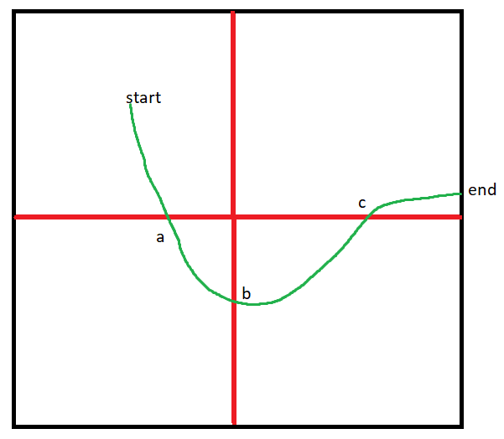
\includegraphics[width=\textwidth/2]{./edge_clips.png}
  \caption{Intersect curve [start,end] with the midlines.
  Sort the intersections parameters together with start, and end into array $u = [start, a,b,c, end]$. Split the curve to sub-curves [start,a], [a,b],[b,c],[c,end].}
  \label{fig:clip}
\end{figure}

Two parameters control the algorithm: tile capacity, \capac~, and the minimal size of a tile: (\mw, \mh).
If for each $(i,j)$ the number of elements in $L_z(i,j).\textit{tiledata}$ is not greater than \capac, or, if $w \leq \mathcal{W}$ and $h \leq \mathcal{H}$, where $w$ ($h$) is the current tile width (correspondengly, height), then the second phase starts.

In our setting \capac~$=500$, and $(\mathcal{W},\mathcal{H}) = 3(w,h)$, where $w$ is the average width and $h$ is the average height of the nodes of the graph.
\subsubsection*{Edge bundling}
In our settings each edge clip is uniquely defined, module direction, by its start and end point. We can use this property to bundle the edges. In each tile we keep a map from unordered pairs of points to the set of edge clips that have these points as start and end points. Each such pair defines an edge bundle. For all edge clips in a bundle we create only one curve segment, avoiding the expensive trimming. We alse count a bundle as one element in the tile, as in most of the cases the drawing attributes of the edges in the bundle are the same.

In our experiments, the number of edge bundles is about 50\% of the number of edge clips, so the edge bundling is a significant optimization.

\subsection*{Second phase of tiling}
The second phase of tiling filters out the entities from the lower layers. We do not change the highest, the most detailed layer.
We sort the nodes of the graph into array $N$ by PageRank~\cite{page1999pagerank}. For each layer $L$, except of the highest, we proceed as follows.
%write pseudo code
\begin{algorithm}
  \begin{algorithmic}[1]
    \Procedure{filter}{$L$}
    \State $r \gets$~\textit{removeEntities}($L$)
    \ForAll{$n$ \textbf{in} $N$}
    \If{!\textit{addNodeToLayer}($n, r, N$)}
    {break}
    \EndIf
    \EndFor
    \EndProcedure
  \end{algorithmic}
\end{algorithm}\\
Here removeEntities}($L$) empties all the tiles of layer $L$, but returns map $r$ allowing to restore the tiles. Function \textit{addNodeToLayer}($n$) returns false and does not change $L$ when one of the tiles intersecting $n$ already has more elements than \capac. Otherwise, the function adds $n$ to all tiles intersected by $n$. It also adds the tile elements for self edges of $n$, and the tile elements for the edges connecting $n$ with the nodes appearing in $N$ before $n$, i.e. the nodes with the rank not lesser than the rank of $n$.

This procedure guarantees that each tile of $L$ has no more than \capac~nodes, but a tile can have more than \capac~ elements in general.
\subsection*{Third phase of tiling}
In the third phase we use a fact that some nodes are not present on the layer. For all layers, except of the highest, we reroute the edges but only around the nodes that are present it the layer. We do not calculate edge routes from scratch, but use the existing routes and only apply the "funnel" heuristic in larger channels.
This gives us simpler edge routes but still has a visual stability during the layer change while browsing.

\section{Future work}
\begin{itemize}
\item Find a tiling method that guarantees that each tile has no more than \capac~elements. One approach could be to use a more aggressive edge bundling to reduce the number of edge clips in the tiles.
\end {itemize}
\bibliography{main}
\bibliographystyle{ieeetr}
\end{document}
